% =========================================================
% CONFIGURACION DEL DOCUMENTO
% =========================================================
\providecommand{\main}{..}
\documentclass[\main/Main.tex]{subfiles}

% =========================================================
% CONTENIDO
% =========================================================
\begin{document}
\chapter{Sistema propuesto}
\label{cha:03_sistema_propuesto}
	% ===============================================================
	% ===============================================================
	\section{\textit{Setup} a utilizar}
	\label{sec:03_setup}
		Debido a que este trabajo de memoria corresponde fundamentalmente a una prueba de concepto se decidió junto al profesor guía evitar en lo posible la compra de nuevo equipamiento y por tanto no se entrega particular importancia a cumplir de forma estricta con las características de \textit{hardware} utilizado en instancias formales de investigación. Con esto en consideración se presenta a continuación una descripción del entorno de trabajo utilizado:
		
		\vspace{-5mm}
		\begin{table}[H]\begin{center}\footnotesize{
			\singlespacing{
			\begin{tabular}{| C{0.11\textwidth} | C{0.13\textwidth} | R{0.16\textwidth} L{0.45\textwidth} |} \hline
				\multirow{8}{*}{Hardware} 	& \multirow{4}{*}{PC} 			& Procesador: 		& Intel Core i7-3770 \\
										& 							& Memoria RAM:		& $16.0[GB]$, DDR3, $650[MHz]$ \\
										& 							& Disco duro: 		& Samsung SSD, 840 Series, $120[GB]$ \\
										& 							& Tarjeta gráfica: 	& NVIDIA GeForce GTX 660 Ti, $2[GB]$ \\ \cline{2-4}
										& \multirow{2}{*}{Monitores}& Principal:		& Samsung SyncMaster, $1680\times1050[px]$, $60[Hz]$ \\ 
										& 							& Secundario: 		& Samsung SyncMaster, $1680\times1050[px]$, $60[Hz]$ \\ \cline{2-4} 
										& Adquisición 				& \textit{Eye tracker}: 		& EyeTribe \\ \cline{2-4}
										& Otro 						& Apoya-barbilla: 	& Hecho a medida\footnotemark. \\ \hline
				\multirow{4}{*}{Software} 	& \multirow{2}{*}{Entorno} 		& SO:				& Windows 10 Pro x64 \\ 
										& 							& Base:				& Python 2.7 x86, Anaconda \\ \cline{2-4}
										& \multirow{2}{*}{Módulos}		& Principal: 			& PsychoPy 1.84.2\cite{psychopy} \\
										& 							& Requeridos:			& Ver anexo \ref{cha:a02_install} \\ \hline
			\end{tabular}}
			\caption{Hardware y software utilizado en el desarrollo.}
			\label{tbl:03_hs_selection}
		}\end{center}\end{table}
		\footnotetext{Diseñado y construido por Christopher Rozas con colaboración del departamento de IDP de la Universidad Técnica Federico Santa María.}

		\newpage
		La elección de software se encuentra influenciada fuertemente por los siguientes puntos:
		\begin{enumerate}\setlength\itemsep{-0.5em}
			\item El \textit{eye tracker} a utilizar solo tiene disponible sus \textit{drivers} para Mac y Windows. Debido a la facilidad de encontrar computadoras con Windows se decanta por este \acrshort{so}.

			\item Los desafíos del sistema a implementar requieren del uso de un lenguaje orientado a objetos. A pesar de las bondades de Octave o Matlab en procesamiento y acceso a módulos complementarios estos entornos carecen de buen soporte para este tipo de programación, por este motivo se utiliza Python como lenguaje de desarrollo. 

			\item Dentro de las opciones disponibles PsychoPy resulta sumamente interesante. Cumple con ser \textit{open-source}, es ampliamente utilizado por investigadores, presenta documentación detallada y clara para todas sus funciones y los foros se encuentran activos. Otro punto interesante es que entrega soporte para varias marcas de \textit{eye tracker}, entre los cuales se encentra el seleccionado.

		\end{enumerate}

	% ===============================================================
	% ===============================================================
	\section{Diseño del sistema}
	\label{sec:03_diseño_sistema}
		El sistema a ser desarrollado en este trabajo de título tiene como función principal facilitar el proceso de configuración y puesta en marcha de experimentos asociados a movimiento ocular. Para esto, se considera oportuno subdividir el desarrollo en tres partes: La primera consiste en determinar la estructura de datos requerida para almacenar tanto las configuraciones del sistema como de las tareas a implementar. La segunda implica la implementación de los métodos de configuración y ejecución del experimento, asegurando su correcto funcionamiento. La tercera etapa corresponde a montar estas funciones en una \textit{GUI} para facilitar el proceso a personas que no tengan conocimiento del lenguaje. Así, se presenta a continuación el trabajo realizado.

		% ###########################################################
		\subsection{Primera parte: Estructura de datos}
		\label{sub:03_estructura_datos}
			Al diseñar la estructura de datos se debió considerar el problema desde tres aristas. La primera correspondía a la necesidad de almacenar la información del conjunto compuesto por experimento-tareas-cuadros-componentes donde, complementando lo expuesto en el apartado \ref{sub:02_experimentos_de_estimulacion}, las tareas corresponden a las actividades específicas que el paciente debe realizar. Los cuadros corresponden a los elementos que conforman dichas tareas y los componentes serán considerados como las figuras e imágenes contenidas en cada cuadro. La segunda dice relación con la información complementaria que se desea incluir para posterior análisis, tal como comentarios del investigador encargado del experimento para una sesión específica o algunas características de quien realizará el experimento, tales como su edad, sexo, color de ojos o si se utilizan lentes durante la ejecución. Finalmente, la tercera arista implica el conservar las configuraciones del equipo y \textit{hardware} a utilizar para montar el servicio de ejecución asociado al módulo \textit{ioHub}, que es el componente de \textit{PsychoPy} que permite sincronizar todos los dispositivos asociados a la ejecución del experimento: teclado, pantalla, \textit{eye tracker}, etc. y almacenar los datos en un archivo. 
			\begin{figure}[H]
				\centering
				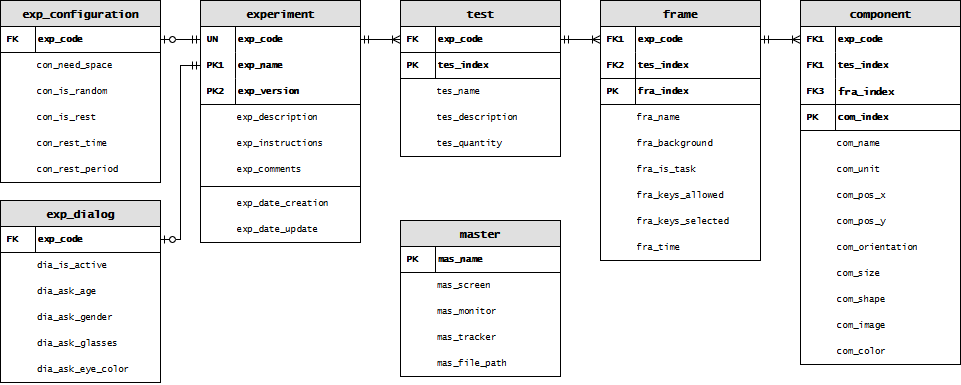
\includegraphics[width=\textwidth]{cap_03_database}
				\caption{Diagrama de base de datos a implementar.}
				\label{fig:03_database}
			\end{figure} 

			En base a lo anterior, se propone como solución el uso de una base de datos local de tipo \textit{SQLite} con la estructura presentada en la figura \ref{fig:03_database}. A continuación se comenta el contenido de cada tabla propuesta y su función:
			\begin{enumerate}\setlength\itemsep{-0.5em}
				\item \textbf{\textref{configuration}:} Almacena la información asociada a un perfil de configuración. Cada perfil se identifica con un nombre (\textref{con\_name}) e indica qué monitor será utilizado (\textref{con\_screen}), cuál es su configuración\footnote{Los parámetros del monitor se definen en un aplicativo especializado de \textit{psychoPy}.} (\textref{con\_monitor}), el \textit{eye tracker} a utilizar (\textref{con\_tracker}) y el directorio en que serán almacenados los resultados (\textref{con\_path}).

				\item \textbf{\textref{experiment}:} Almacena la configuración de un experimento. Cada experimento se identifica por un código único (\textref{exp\_code}) y un par nombre / versión (\textref{exp\_name} / \textref{exp\_version}), que tiene como objetivo identificar a una aplicación específica de una familia del mismo tipo, por ejemplo: (''antisaccade'' / ''v1.0''). Además, se incluye un campo para indicar una descripción (\textref{exp\_description}), instrucciones para el usuario (\textref{exp\_instructions}) y comentarios para quien tome el experimento (\textref{exp\_comments}). Se incluyen la fecha de creación y la última modificación para dejar de forma explícita una señal de cuidado: Las condiciones del experimento pueden no ser las mismas de la última ejecución.
				
				\item \textbf{\textref{exp\_configuration}:} Esta tabla es complementaria al experimento y almacena la configuración general de ejecución. \textquestiondown Es necesario que el paciente presione la tecla espacio antes de cada tarea? (\textref{exp\_need\_space}), \textquestiondown El orden de las tareas es aleatorio o secuencial? (\textref{exp\_is\_random}), \textquestiondown Se incluyen en el experimento tiempos de descanso? (\textref{exp\_is\_rest}), \textquestiondown Cada cuántas tareas? (\textref{exp\_rest\_period}), \textquestiondown Con qué duración? (\textref{exp\_rest\_time}).

				\item \textbf{\textref{exp\_dialog}:} Esta tabla es complementaria al experimento y almacena la configuración del diálogo inicial, que permite obtener información adicional sobre el paciente. \textquestiondown Es necesario incluir información complementaria? (\textref{dia\_is\_active}), \textquestiondown Qué edad tiene el paciente? (\textref{dia\_ask\_age}), \textquestiondown Cuál es su sexo? (\textref{dia\_ask\_gender}), \textquestiondown Utiliza gafas o lentes de contacto? (\textref{dia\_ask\_glasses}), \textquestiondown Cuál es su color de ojos? (\textref{dia\_ask\_eye\_color}).

				\item \textbf{\textref{test}:} Almacena, para cada experimento, la identificación de las tareas que lo componen ordenadas por un índice (\textref{tes\_index}). Cada tarea se identifica por su nombre (\textref{tes\_name}), que es único para cada experimento, y un campo para añadir su descripción (\textref{tes\_description}).

				\item \textbf{\textref{exp\_sequence}:} Almacena, para cada experimento, la secuencia de tareas a ejecutar. Cada ítem incluye un identificador del experimento (\textref{exp\_code}) y la tarea correspondiente (\textref{tes\_index}), además de un índice que permite definir el orden de ejecución (\textref{seq\_index}) y el número de veces que debe ejecutarse la tarea (\textref{seq\_quantity}). 

				\item \textbf{\textref{frame}:} Esta tabla contiene, para cada tarea, el conjunto de cuadros que la conforman ordenados por aparición mediante un índice (\textref{fra\_index}). Cada cuadro se identifica por un nombre (\textref{fra\_name}),  único para cada tarea, y permite la configuración de su comportamiento y características de forma general: color de fondo (\textref{fra\_color}), si el cuadro corresponde a una tarea que requiere respuesta de teclado o es temporizada (\textref{fra\_is\_task}), las teclas habilitadas (\textref{fra\_keys\_allowed}) y las teclas que se espera sean presionadas (\textref{fra\_keys\_correct}) en el primer caso o el tiempo por el cual debe ser presentado (\textref{fra\_time}) en el segundo.

				\item \textbf{\textref{component}:} Esta tabla contiene, para cada cuadro, el conjunto de componentes o elementos que lo conforman ordenados por presentación mediante un índice (\textref{com\_index}). Cada componente se identifica por un nombre (\textref{com\_name}), único para cada cuadro, y las configuraciones asociadas tanto a las unidades de medida a utilizar (\textref{com\_units}), su posición en la pantalla ((\textref{com\_pos\_x}), (\textref{com\_pos\_y})), su tamaño (\textref{com\_size}), si se encuentra rotada o no (\textref{com\_rotation}), en el cao de ser figura su forma (\textref{com\_shape}) y color (\textref{com\_color}) o si es una imagen la información binaria correspondiente (\textref{com\_image}). 
			\end{enumerate}

			Este modelo se considera apropiado por los siguientes motivos:
			\begin{enumerate}\setlength\itemsep{-0.5em}
				\item Aísla un experimento de otro al tener tareas y configuraciones completamente independientes. Esta configuración permite evitar que cambios en alguna tarea específicas afecte a mas de un experimento.

				\item No puede existir una tarea que no se encuentre asociada a un experimento, lo que evita almacenar datos innecesarios (esto aplica también a cuadros y componentes). 

				\item Tener todas las configuraciones almacenadas en un archivo facilita la portabilidad y migración desde un equipo a otro. Además, dado que es tratable como una base de datos convencional facilita el proceso de revisión de los datos sin necesidad de contar con el programa principal.
			\end{enumerate}

			Cabe destacar que, para asegurar la limpieza de la base de datos se tomo la decisión de definir las operaciones de \textit{update} como \textit{delete} en cascada a todas las tablas asociadas a un experimento. Esto implica que al eliminar un experimento particular también se eliminan todos los datos dependientes de él, tales como sus tareas, cuadros y componentes, evitando mantener data residual. Cabe destacar que esto se define también en niveles más bajos: Remover una tarea elimina todos sus cuadros, si es un cuadro se eliminan todos sus componentes.  

		% ###########################################################
		\subsection{Segunda parte: Implementación de las funciones principales}
		\label{sub:03_implementacion_backtend}
			Para lograr sincronizar la ejecución del experimento con el uso de dispositivos tales como el monitor, teclado y \textit{eye tracker} se hará uso de \textit{ioHub} \cite{website:iohub}. Esta herramienta, que forma parte de los módulos de \textit{psychoPy}, tiene por característica principal la capacidad de montar un servicio que permite realizar una revisión constante de los dispositivos de entrada/salida configurados previamente para el experimento, almacenando la información recopilada de forma ordenada en un archivo con formato \textit{hdf5}. Este tipo de archivos es considerado estándar en investigación y, a grandes rasgos, corresponde a un tipo \textit{\gls{log}} de datos organizado a modo de diccionario. Utilizando esta aplicación se plantea formular un sistema que permita las funcionalidades presentadas en la figura \ref{fig:03_application_concept}. 

			La aplicación propuesta tiene por requerimientos tanto la configuración del experimento (\textref{Experiment}) como la del perfil de configuración (\textref{Configuration Profile}), explicados en la sección \ref{sub:03_estructura_datos}.

			\begin{figure}[H]
				\centering
				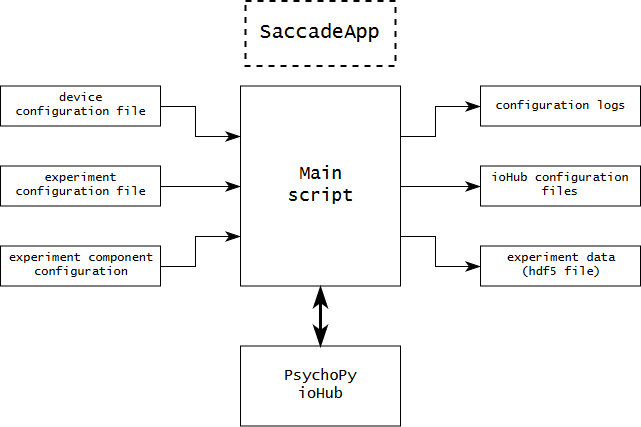
\includegraphics[width=0.8\textwidth]{cap_03_application_concept}
				\caption{Diagrama de funcionamiento general.}
				\label{fig:03_application_concept}
			\end{figure} 

			Los resultados esperados son:
			\begin{enumerate}\setlength\itemsep{-0.5em}
				\item Creación de una estructura de carpetas que permita almacenar la información de las distintas instancias de ejecución de forma organizada y clara. 

				Para lograr esto se propone el sistema de la figura \ref{fig:03_folder_structure} que consiste en separar los resultados por tipo de experimento y por versión. De esta forma, en el directorio base determinado en el perfil de configuración (\textref{Base\_Folder}) se crean carpetas con los nombres de los experimentos ejecutados (\textref{Experiment\_Name}) y dentro de estas se organizan los resultados en carpetas que indican la versión del experimento (\textref{Experiment\_Version}) y su código (\textref{Experiment\_Code}).  
				\begin{figure}[H]
					\centering
					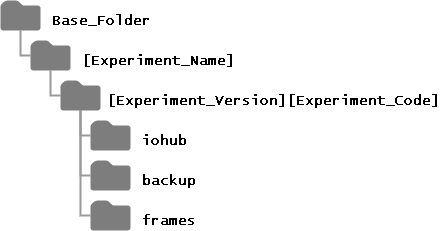
\includegraphics[width=0.6\textwidth]{cap_03_folder_structure}
					\caption{Estructura de directorios para resultados.}
					\label{fig:03_folder_structure}
				\end{figure} 

				\item Para facilitar el proceso de revisión y posterior \textit{debug} de los experimentos realizados se decide almacenar en la carpeta de resultados 3 archivos: El primer archivo, a almacenar en la carpeta \textref{backup} consiste en un diccionario que contiene todas las configuraciones asociadas al experimento y perfil utilizados (\textref{Backup Configuration File}). Los siguientes 2 archivos, a almacenar en la carpeta \textref{ioHub}, corresponden a las configuraciones del experimento y \textit{hardware} en el formato requerido por \textit{ioHub} para su funcionamiento (\textref{ioHub Configuration Files}). Para identificar una ejecución de otra, cada grupo de archivos se identifica por la marca de tiempo del momento de ejecución en formato \textit{Unix}.

				\item Los resultados del experimento (\textref{Experiment Data}) se almacenan directamente en la carpeta \textref{[Experiment\_Version][Experiment\_Code]}. Este archivo se actualiza con cada ejecución y contiene los resultados de todas las sesiones del experimento. 

				\item De forma opcional, el \textit{script} permite obtener capturas de pantalla de cada uno de los cuadros del experimento (\textref{Frame Images}). Estas imágenes son almacenadas en la carpeta \textref{frames}. 
			\end{enumerate}

			En la figura \ref{fig:03_base_class_tree} se presenta la estructura de clases implementada en este trabajo de título. Las clases \textref{Configuration}, \textref{Experiment}, \textref{Test}, \textref{Frame} y \textref{Component} representan el conjunto de métodos que permiten la manipulación de los datos almacenados en la base de datos, además de entregar funcionalidades que permiten la ejecución. 
			\begin{figure}[H]
				\centering
				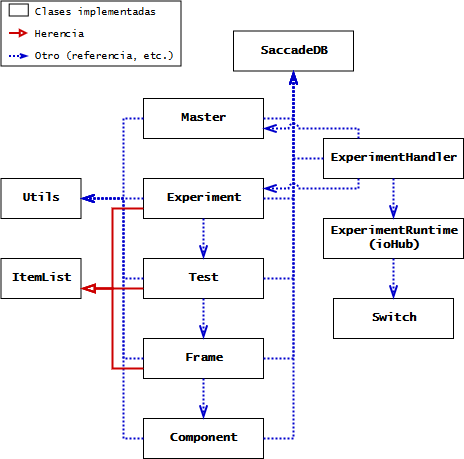
\includegraphics[width=\textwidth]{cap_03_base_class_tree}
				\caption{Diagrama de clases del sistema (no considera \textit{GUI}).}
				\label{fig:03_base_class_tree}
			\end{figure} 

			Debido a que las clases \textref{Experiment}, \textref{Test} y \textref{Frame} implican el manejo de una lista de objetos se crea una clase base llamada \textref{ItemList} que permite integrar funcionalidades tales como agregar, quitar, mover o reemplazar elementos. Además, ya que un experimento implica la ejecución de una secuencia de tareas que pueden repetirse se implementa una variante de \textref{ItemList} que permite la manipulación de secuencias en base a los elementos disponibles en lista \textref{ItemListSequence}.

			Las clases \textref{SaccadeDB} y \textref{Switch} añaden funcionalidades transversales al resto de las clases: \textref{SaccadeDB} permite la comunicación e interacción con el archivo de base de datos y \textref{Switch} permite implementar estructuras \textit{switch-case} para facilitar el uso de máquinas de estado. \textref{ExperimentHandler} y \textref{ExperimentRuntime} (que hereda sus funcionalidades de \textref{ioHub} e inicializa los servicios asociados) son las encargadas de preparar los archivos de configuración y ejecutar el experimento respectivamente.   

			En las siguientes páginas se procede a describir con un mayor grado de detalle cada clase y módulo utilizado. Por simplicidad se obvian las funciones asociadas al get-set de los atributos de las clases (ya que corresponden a los datos almacenados en la base de datos).
			
			\begin{enumerate}\setlength\itemsep{-0.5em}
				\item \textbf{\textref{utils}:} Módulo auxiliar que implementa métodos de uso general.
				
				\vspace{-8mm}			
				\begin{center}\footnotesize{\singlespacing{
					\begin{longtable}[H]{| C{0.12\textwidth} | R{0.16\textwidth} L{0.6\textwidth} |} \hline
						% ===============================================
						\multicolumn{3}{|c|}{\textbf{\textref{format\_text}}}\\\hline
						Descripción & \multicolumn{2}{L{0.75\textwidth}|}{
						Convierte el dato de entrada a unicode. Si el dato ingresado no cumple con las condiciones de formato se levanta una excepción indicando el error asociado.
						}\\\hline
						\multirow{4}{*}{Inputs}	& text: 			& Dato a ser convertido en \textref{unicode}. \\
						 						& lmin: 			& Largo mínimo (\textref{int}). Por defecto: \textref{None} (Sin condición). \\
						 						& lmax: 			& Largo máximo (\textref{int}). Por defecto: \textref{None} (Sin condición)\\
						 						& var\_name:		& Nombre de la variable para la cual se utilizará el dato formateado (\textref{string}). Se agrega en el mensaje de excepción para hacer seguimiento del error. Por defecto: vacío (Sin nombre).
						\\\hline
						Return 					& \textref{unicode}.& 
						\\\hline 
						% ===============================================
						\multicolumn{3}{|c|}{\textbf{\textref{format\_int}}}\\\hline
						Descripción & \multicolumn{2}{L{0.75\textwidth}|}{
						Convierte un valor de entrada en entero. Si el valor ingresado no cumple con las condiciones de formato se levanta una excepción indicando el error asociado.
						} \\ \hline
						\multirow{4}{*}{Inputs} & value: 			& Valor a ser convertido en int. \\
						 						& vmin: 			& Valor mínimo permitido (\textref{int}). Por defecto: \textref{None} (Sin condición)\\
						 						& vmax: 			& Valor máximo permitido (\textref{int}). Por defecto: \textref{None} (Sin condición)\\
						 						& var\_name:		& Nombre de la variable para la cual se utilizará el dato formateado (\textref{string}). Se agrega en el mensaje de excepción para hacer seguimiento del error. Por defecto: vacío (Sin nombre). 
						\\\hline
						Return 					& \textref{int}. 	& 
						\\\hline \newpage
						% ===============================================
						\multicolumn{3}{|c|}{\textbf{\textref{format\_float}}}\\\hline
						Descripción & \multicolumn{2}{L{0.75\textwidth}|}{
						Convierte un valor de entrada en flotante. Si el valor ingresado no cumple con las condiciones de formato se levanta una excepción indicando el error asociado.
						}\\\hline
						\multirow{4}{*}{Inputs} & value: 			& Valor a ser convertido en float. \\
						 						& vmin: 			& Valor mínimo permitido (\textref{float}). Por defecto: \textref{None} (Sin condición)\\
						 						& vmax: 			& Valor máximo permitido (\textref{float}). Por defecto: \textref{None} (Sin condición)\\
						 						& var\_name:		& Nombre de la variable para la cual se utilizará el dato formateado (\textref{string}). Se agrega en el mensaje de excepción para hacer seguimiento del error. Por defecto: vacío (Sin nombre).
						\\\hline
						Return 					& \textref{float}. 	& 
						\\\hline
						% ===============================================
						\multicolumn{3}{|c|}{\textbf{\textref{format\_bool}}}\\\hline
						Descripción & \multicolumn{2}{L{0.75\textwidth}|}{
						Convierte el valor de entrada entregado en un booleano. Si el dato ingresado no puede ser convertido se levanta una excepción indicando el error asociado.
						}\\\hline
						\multirow{2}{*}{Inputs} & state: 			& Variable a convertir en bool. \\
						 						& var\_name:		& Nombre de la variable para la cual se utilizará el dato formateado (\textref{string}). Se agrega en el mensaje de excepción para hacer seguimiento del error. Por defecto: vacío (Sin nombre).
						\\\hline
						Return 					& \textref{bool}. 	& 
						\\ \hline 
						% ===============================================
						\multicolumn{3}{|c|}{\textbf{\textref{is\_in\_list}}}\\\hline
						Descripción & \multicolumn{2}{L{0.75\textwidth}|}{
						Indica si un elemento se encuentra o no en una lista.
						}\\\hline
						\multirow{2}{*}{Inputs} & item: 			& Elemento a encontrar. \\
												& item\_list:		& Lista a revisar (\textref{list}). 
						\\\hline
						Return 					& \textref{bool}. 	&  \textref{True} en caso de ser encontrado, \textref{False} en caso contrario.
						\\\hline 
						% ===============================================
						\multicolumn{3}{|c|}{\textbf{\textref{get\_time}}}\\\hline
						Descripción & \multicolumn{2}{L{0.75\textwidth}|}{
						Permite convertir una fecha desde el formato de tiempo GTM al horario de Chile continental.
						}\\\hline
						Inputs 					& date: 			& Fecha (\textref{string}) en formato ''\textref{Y-m-d H:M:S}''. 
						\\\hline
						Return 					& \textref{unicode}.& 
						\\\hline
						% ===============================================
						\multicolumn{3}{|c|}{\textbf{\textref{get\_main\_path}}}\\\hline
						Descripción & \multicolumn{2}{L{0.75\textwidth}|}{
						Retorna la ubicación en donde la aplicación se encuentra siendo ejecutada. 
						}\\\hline
						Inputs 					& \textref{void}. 	& 
						\\\hline
						Return 					& \textref{unicode}.& 
						\\\hline
						% ===============================================
						\multicolumn{3}{|c|}{\textbf{\textref{get\_module\_path}}}\\\hline
						Descripción & \multicolumn{2}{L{0.75\textwidth}|}{
						Retorna la ubicación donde se encuentra almacenado el módulo de la aplicación (\textref{saccadeapp}).
						}\\\hline
						Inputs 					& \textref{void}. 	&  
						\\\hline
						Return 					& \textref{unicode}.& 
						\\\hline
						% ===============================================
						\multicolumn{3}{|c|}{\textbf{\textref{format\_path}}}\\\hline
						Descripción & \multicolumn{2}{L{0.75\textwidth}|}{
						Modifica la ubicación de entrada dependiendo del sistema operativo para asegurar compatibilidad. 
						}\\\hline
						Inputs 					& path: 			& Ubicación de un archivo o directorio (\textref{string}). 
						\\\hline
						Return 					& \textref{bool}. 	& 
						\\\hline \newpage
						% ===============================================
						\multicolumn{3}{|c|}{\textbf{\textref{get\_available\_colors}}}\\\hline
						Descripción & \multicolumn{2}{L{0.75\textwidth}|}{
						Retorna una lista con los nombres de los colores disponibles en \textit{psychoPy}.
						}\\\hline
						Inputs 					& \textref{void}. 	& 
						\\\hline
						Return 					& \textref{list}. 	& Si no hay elementos: lista vacía.
						\\\hline
						% ===============================================
						\multicolumn{3}{|c|}{\textbf{\textref{get\_available\_trackers}}}\\\hline
						Descripción & \multicolumn{2}{L{0.75\textwidth}|}{
						Retorna una lista con los nombres de los \textit{eye trackers} disponibles.
						}\\\hline
						Inputs 					& \textref{void}. 	& 
						\\\hline
						Return 					& \textref{list}. 	& Si no hay elementos: lista vacía.
						\\\hline
						% ===============================================
						\multicolumn{3}{|c|}{\textbf{\textref{get\_available\_screens}}}\\\hline
						Descripción & \multicolumn{2}{L{0.75\textwidth}|}{
						Retorna una lista con la información (id y resolución) de los monitores disponibles.
						}\\\hline
						Inputs 					& \textref{void}. 	& 
						\\\hline
						Return 					& \textref{list}. 	& Si no hay elementos: lista vacía.
						\\\hline
						% ===============================================
						\multicolumn{3}{|c|}{\textbf{\textref{get\_available\_monitors}}}\\\hline
						Descripción & \multicolumn{2}{L{0.75\textwidth}|}{
						Retorna una lista con los nombres de los perfiles de configuración de monitor disponibles en \textit{psychoPy} mediante el \textit{Monitor Center}.
						}\\\hline
						Inputs 					& \textref{void}. 	& 
						\\\hline
						Return 					& \textref{list}. 	& Si no hay elementos: lista vacía. 
						\\\hline 
						% ===============================================
						\multicolumn{3}{|c|}{\textbf{\textref{get\_available\_units}}}\\\hline
						Descripción & \multicolumn{2}{L{0.75\textwidth}|}{
						Retorna una lista con los nombres de los tipos de unidad disponibles en \textit{psychoPy} para el dibujo de estímulos en pantalla.
						}\\\hline
						Inputs 					& \textref{void}. 	& 
						\\\hline
						Return 					& \textref{list}. 	& Si no hay elementos: lista vacía. 
						\\\hline
						% ===============================================
						\multicolumn{3}{|c|}{\textbf{\textref{get\_available\_shapes}}}\\\hline
						Descripción & \multicolumn{2}{L{0.75\textwidth}|}{
						Retorna una lista con los nombres de las figuras disponibles para la construcción de estímulos.
						}\\\hline
						Inputs 					& \textref{void}. 	& 
						\\\hline
						Return 					& \textref{list}. 	& Si no hay elementos: lista vacía.
						\\\hline
						% ===============================================
						\multicolumn{3}{|c|}{\textbf{\textref{open\_documentation}}}\\\hline
						Descripción & \multicolumn{2}{L{0.75\textwidth}|}{
						Abre una copia del documento de memoria como documentación.
						}\\\hline
						Inputs 					& \textref{void}. 	& 
						\\\hline
						Return 					& \textref{void}. 	& 
						\\\hline
						% ===============================================
						\multicolumn{3}{|c|}{\textbf{\textref{open\_psychopy\_monitor\_center}}}\\\hline
						Descripción & \multicolumn{2}{L{0.75\textwidth}|}{
						Abre una instancia de la aplicación de configuración de monitores de \textit{psychoPy}.
						}\\\hline
						Inputs 					& \textref{void}. 	& 
						\\\hline
						Return 					& \textref{bool}. 	&  \textref{True} si abre una nueva ventana, \textref{False} si ya existe una en ejecución. 
						\\\hline
					\caption{Métodos implementados en \textref{utils}.}
					\label{tbl:03_class_utils}
					\end{longtable}}}
				\end{center}

				\newpage
				\item \textbf{\textref{SaccadeDB}:} Clase utilizada para implementar la conexión con la base de datos SQLite.
				
				\vspace{-8mm}			 
				\begin{center}\footnotesize{\singlespacing{
					\begin{longtable}[H]{| C{0.12\textwidth} | R{0.16\textwidth} L{0.6\textwidth} |} \hline
						% ===============================================
						\multicolumn{3}{|c|}{\textbf{\textref{SaccadeDB}}}\\\hline
						Descripción & \multicolumn{2}{L{0.75\textwidth}|}{
						Constructor. Inicializa los atributos del objeto.
						}\\\hline
						Inputs 					& path: 			& Directorio en donde se encuentra el archivo de base de datos (\textref{string}). Por defecto: vacío (Se crea en el directorio de ejecución).
						\\\hline
						Return 					& \textref{void}. 	& 
						\\\hline 
						% ===============================================
						\multicolumn{3}{|c|}{\textbf{\textref{connect}}}\\\hline
						Descripción & \multicolumn{2}{L{0.75\textwidth}|}{
						Inicia una conexión con el archivo de base de datos. Si el archivo de base de datos epecificado en el constructor no existe, crea uno nuevo.
						}\\\hline
						Inputs 					& \textref{void}. 	&  
						\\\hline
						Return 					& \textref{void}. 	& 
						\\\hline 
						% ===============================================
						\multicolumn{3}{|c|}{\textbf{\textref{close}}}\\\hline
						Descripción & \multicolumn{2}{L{0.75\textwidth}|}{
						Finaliza, de ser posible, la conexión con la base de datos.
						}\\\hline
						Inputs 					& \textref{void}. 	&  
						\\\hline
						Return 					& \textref{bool}. 	& \textref{True} si la acción se realizó correctamente, \textref{False} en caso contrario.
						\\\hline
						% ===============================================
						\multicolumn{3}{|c|}{\textbf{\textref{push\_query}}}\\\hline
						Descripción & \multicolumn{2}{L{0.75\textwidth}|}{
						Permite realizar querys para modificar los contenidos de la base de datos (\textref{insert, update, delete}).
						}\\\hline
						Inputs 					& query. 			& Instrucción SQL (\textref{string}).
						\\\hline
						Return 					& \textref{bool}. 	& \textref{True} si la acción se realizó correctamente, \textref{False} en caso contrario.
						\\\hline 
						% ===============================================
						\multicolumn{3}{|c|}{\textbf{\textref{pull\_query}}}\\\hline
						Descripción & \multicolumn{2}{L{0.75\textwidth}|}{
						Permite realizar querys para obtener datos desde de la base de datos (\textref{select}).
						}\\\hline
						Inputs 					& query. 			& Instrucción SQL (\textref{string}).
						\\\hline
						Return 					& \textref{object}. & Array (\textref{numpy}) en caso de existir datos, \textref{None} en caso contrario. 
						\\\hline 
					\caption{Métodos implementados en la clase \textref{SaccadeDB}.}
					\label{tbl:03_class_saccadedb}
					\end{longtable}}}
				\end{center}

				\vspace{-15mm}

				\item \textbf{\textref{Configuration}:} Clase que permite manipular las configuración del \textit{hardware} a utilizar en la ejecución de un experimento y la ubicación de los archivos de salida de la misma. Para utilizar las funciones de carga/guardado es necesario asignar un objeto de base de datos  (\textref{SaccadeDB}). 
				
				\vspace{-8mm}
				\begin{center}\footnotesize{\singlespacing{
					\begin{longtable}[H]{| C{0.12\textwidth} | R{0.16\textwidth} L{0.6\textwidth} |} \hline
						% ===============================================
						\multicolumn{3}{|c|}{\textbf{\textref{Configuration}}}\\\hline
						Descripción & \multicolumn{2}{L{0.75\textwidth}|}{
						Constructor. Inicializa los atributos del objeto. Si se le entrega una objeto de base de datos y un nombre (asociado a un perfil de configuración) carga inmediatamente los datos. 
						}\\\hline
						\multirow{2}{*}{Inputs} & db: 				& Instancia de clase (\textref{SaccadeDB}). Por defecto: vacío. (Sin conexión). \\
						 						& name: 			& Nombre de perfil de configuración (\textref{string}). Por defecto: vacío (No buscar).
						\\\hline
						Return 					& \textref{void}. 	& 
						\\\hline \newpage
						% ===============================================
						\multicolumn{3}{|c|}{\textbf{\textref{get\_list}}}\\\hline
						Descripción & \multicolumn{2}{L{0.75\textwidth}|}{
						Método estático. Entrega una lista con los nombres de los perfiles de configuración que se encuentran almacenados en la base de datos.
						}\\\hline
						Inputs 					& db: 				& Instancia de clase (\textref{SaccadeDB}). Por defecto: vacío. (Sin conexión). 
						\\\hline
						Return 					& \textref{list}.	& Si no hay elementos: lista vacía.
						\\\hline 
						% ===============================================
						\multicolumn{3}{|c|}{\textbf{\textref{load}}}\\\hline
						Descripción & \multicolumn{2}{L{0.75\textwidth}|}{
						Permite cargar en el objeto las configuraciones almacenadas en la base de datos.
						}\\\hline
						Inputs 					& name: 			& Nombre de perfil de configuración (\textref{string}).
						\\\hline
						Return 					& \textref{bool}.	& \textref{True} si la acción se realizó correctamente, \textref{False} en caso contrario.
						\\\hline 
						% ===============================================
						\multicolumn{3}{|c|}{\textbf{\textref{save}}}\\\hline
						Descripción & \multicolumn{2}{L{0.75\textwidth}|}{
						Permite guardar el perfil de configuración en la base de datos.
						}\\\hline
						Inputs 					& \textref{void}. 	& 
						\\\hline
						Return 					& \textref{bool}.	& \textref{True} si la acción se realizó correctamente, \textref{False} en caso contrario.
						\\\hline 
						% ===============================================
						\multicolumn{3}{|c|}{\textbf{\textref{copy}}}\\\hline
						Descripción & \multicolumn{2}{L{0.75\textwidth}|}{
						Permite realizar una copia del objeto siempre que el nombre asignado no exista en la base de datos.
						}\\\hline
						Inputs 					& name: 			& Nombre a ser asignado en la copya del perfil de configuración (\textref{string}).
						\\\hline
						Return 					& \textref{object}.	& Devuelve una copia si se ingresa un nombre correctamente, \textref{None} en caso contrario.
						\\\hline 
						% ===============================================
						\multicolumn{3}{|c|}{\textbf{\textref{remove}}}\\\hline
						Descripción & \multicolumn{2}{L{0.75\textwidth}|}{
						Permite eliminar el perfil de configuración de la base de datos.
						}\\\hline
						Inputs 					& \textref{void}. 	& 
						\\\hline
						Return 					& \textref{bool}.	& \textref{True} si la acción se realizó correctamente, \textref{False} en caso contrario.
						\\\hline 
						% ===============================================
						\multicolumn{3}{|c|}{\textbf{\textref{get\_iohub}}}\\\hline
						Descripción & \multicolumn{2}{L{0.75\textwidth}|}{
						Retorna un diccionario con las configuraciones y formatos requeridos por \textit{ioHub} para definir los dispositivos de \textit{hardware} a ser utilizados en la ejecución de un experimento.
						}\\\hline
						Inputs 					& \textref{void}. 	& 
						\\\hline
						Return 					& \textref{dict}.	& Si no existe en la base de datos: \textref{None}.
						\\\hline
						\multicolumn{3}{|c|}{\textbf{\textref{get\_configuration}}}\\\hline
						Descripción & \multicolumn{2}{L{0.75\textwidth}|}{
						Retorna un diccionario que contiene los atributos del objeto.
						}\\\hline
						Inputs 					& \textref{void}. 	& 
						\\\hline
						Return 					& \textref{dict}.	& Si no existe en la base de datos: \textref{None}.
						\\\hline
					\caption{Métodos implementados en la clase \textref{Configuration}.}
					\label{tbl:03_class_configuration}
					\end{longtable}}}
				\end{center}

				\newpage
				\item \textbf{\textref{ItemList}:} Clase utilizada para manejar listas de objetos. Su implementación no considera el uso directo por parte de los usuarios del programa.

				\vspace{-8mm}
				\begin{center}\footnotesize{\singlespacing{
					\begin{longtable}[H]{| C{0.12\textwidth} | R{0.16\textwidth} L{0.6\textwidth} |} \hline
						% ===============================================
						\multicolumn{3}{|c|}{\textbf{\textref{ItemList}}}\\\hline
						Descripción & \multicolumn{2}{L{0.75\textwidth}|}{
						Constructor. Inicializa los atributos de la clase. Permite definir el tipo de objetos a manipular. 
						}\\\hline
						Inputs 					& item\_class:		& Tipo de objeto (\textref{Test}, \textref{Frame}, \textref{Component}).
						\\\hline
						Return 					& \textref{void}. 	& 
						\\\hline 
						% ===============================================
						\multicolumn{3}{|c|}{\textbf{\textref{item\_add}}}\\\hline
						Descripción & \multicolumn{2}{L{0.75\textwidth}|}{
						Permite agregar un objeto a la lista. 
						}\\\hline
						Inputs 					& item: 			& Objeto a añadir (\textref{item\_class}).
						\\\hline
						Return 					& \textref{bool}.	& \textref{True} si el objeto fue añadido, \textref{False} si el objeto es del tipo definido.
						\\\hline 
						% ===============================================
						\multicolumn{3}{|c|}{\textbf{\textref{item\_copy}}}\\\hline
						Descripción & \multicolumn{2}{L{0.75\textwidth}|}{
						Agrega una copia del objeto seleccionado en el último lugar de la lista.
						}\\\hline
						\multirow{2}{*}{Inputs}	& item\_id: 		& Posición en lista del objeto a copiar (\textref{int}). \\
												& name:				& Nombre del nuevo objeto (\textref{string}). 
						\\\hline
						Return 					& \textref{bool}.	& \textref{True} si el índice existe y se realiza la copia, \textref{False} en caso contrario.
						\\\hline 
						% ===============================================
						\multicolumn{3}{|c|}{\textbf{\textref{item\_remove}}}\\\hline
						Descripción & \multicolumn{2}{L{0.75\textwidth}|}{
						Elimina el objeto seleccionado.
						}\\\hline
						Inputs 					& item\_id: 		& Posición en lista del objeto a eliminar (\textref{int}).
						\\\hline
						Return 					& \textref{bool}.	& \textref{True} si el índice existe y es eliminado, \textref{False} en caso contrario.
						\\\hline 
						% ===============================================
						\multicolumn{3}{|c|}{\textbf{\textref{item\_replace}}}\\\hline
						Descripción & \multicolumn{2}{L{0.75\textwidth}|}{
						Remplaza el objeto seleccionado por uno nuevo.
						}\\\hline
						\multirow{2}{*}{Inputs}	& item\_id: 		& Posición en lista del objeto a reemplazar (\textref{int}). \\
												& new\_item:		& Objeto reemplazante (\textref{item\_class}). 
						\\\hline
						Return 					& \textref{bool}.	& \textref{True} si el índice existe y el objeto es añadido, \textref{False} en caso contrario.
						\\\hline 
						% ===============================================
						\multicolumn{3}{|c|}{\textbf{\textref{item\_swap}}}\\\hline
						Descripción & \multicolumn{2}{L{0.75\textwidth}|}{
						Permite hacer un enroque entre dos elementos de la lista.
						}\\\hline
						\multirow{2}{*}{Inputs}	& item1\_id: 		& Posición en lista del primer objeto (\textref{int}). \\
												& item2\_id:		& Posición en lista del segundo objeto (\textref{int}). 
						\\\hline
						Return 					& \textref{bool}.	& \textref{True} si los índices existen y se realiza el enroque, \textref{False} en caso contrario.
						\\\hline
						% ===============================================
						\multicolumn{3}{|c|}{\textbf{\textref{get\_items}}}\\\hline
						Descripción & \multicolumn{2}{L{0.75\textwidth}|}{
						Retorna la lista de objetos.
						}\\\hline
						Inputs 					& \textref{void}. 	& 
						\\\hline
						Return 					& \textref{list}.	& Si no hay elementos: lista vacía.
						\\\hline
						% ===============================================
						\multicolumn{3}{|c|}{\textbf{\textref{get\_item}}}\\\hline
						Descripción & \multicolumn{2}{L{0.75\textwidth}|}{
						Retorna un elemento de la lista en base a su índice. 
						}\\\hline
						Inputs 					& item\_id:			& Posición en lista del objeto a recuperar (\textref{int}). 
						\\\hline
						Return 					& \textref{object}.	& Si el índice no existe: \textref{None}. 
						\\\hline \newpage
						% ===============================================
						\multicolumn{3}{|c|}{\textbf{\textref{check\_item\_name}}}\\\hline
						Descripción & \multicolumn{2}{L{0.75\textwidth}|}{
						Retorna el índice del objeto que tenga el nombre ingresado.  
						}\\\hline
						Inputs 					& item\_name: 		& Nombre del objeto a buscar (\textref{string}).  
						\\\hline
						Return 					& \textref{int}.	& Si el nombre no existe: -1. 
						\\\hline
						% ===============================================
						\multicolumn{3}{|c|}{\textbf{\textref{get\_items\_str}}}\\\hline
						Descripción & \multicolumn{2}{L{0.75\textwidth}|}{
						Retorna una lista con los nombres de los objetos almacenados.  
						}\\\hline
						Inputs 					& \textref{void}. 	& 
						\\\hline
						Return 					& \textref{list}.	& Si no hay elementos: lista vacía
						\\\hline
						% ===============================================
						\multicolumn{3}{|c|}{\textbf{\textref{get\_items\_length}}}\\\hline
						Descripción & \multicolumn{2}{L{0.75\textwidth}|}{
						Devuelve el número de elementos de la lista. 
						}\\\hline
						Inputs 					& \textref{void}. 	&  
						\\\hline
						Return 					& \textref{int}.	&
						\\\hline
					\caption{Métodos implementados en la clase \textref{ItemList}.}
					\label{tbl:03_class_itemlist}
					\end{longtable}}}
				\end{center}

				\vspace{-15mm}

				\item \textbf{\textref{ItemListSequence}:} Clase utilizada para extender las capacidades de una lista de objetos (hija de \textref{ItemList}) permitiendo la configuración y manejo de secuencias. Para su funcionamiento deben re-implementarse dos métodos: El primero es \textref{item\_remove} ya que debe incluirse la eliminación de los elementos de la secuencia asociados al item. El segundo es \textref{item\_replace} ya que deben actualizarse las referencias de los elementos de la secuencia al nuevo ítem.  

				\vspace{-8mm}
				\begin{center}\footnotesize{\singlespacing{
					\begin{longtable}[H]{| C{0.12\textwidth} | R{0.16\textwidth} L{0.6\textwidth} |} \hline
						% ===============================================
						\multicolumn{3}{|c|}{\textbf{\textref{ItemListSequence}}}\\\hline
						Descripción & \multicolumn{2}{L{0.75\textwidth}|}{
						Constructor. Inicializa los atributos de la clase. Permite definir el tipo de objetos a manipular. 
						}\\\hline
						Inputs 					& item\_class:		& Tipo de objeto (\textref{Test}, \textref{Frame}, \textref{Component}).
						\\\hline
						Return 					& \textref{void}. 	& 
						\\\hline 
						% ===============================================
						\multicolumn{3}{|c|}{\textbf{\textref{sequence\_add}}}\\\hline
						Descripción & \multicolumn{2}{L{0.75\textwidth}|}{
						Permite agregar un elemento a la secuencia. 
						}\\\hline
						\multirow{2}{*}{Inputs}	& item\_id: 		& Posición en lista del objeto a agregar (\textref{int}). \\
												& quantity:			& Cantidad de veces que será ejecutado (\textref{int}).
						\\\hline
						Return 					& \textref{bool}.	& \textref{True} si el índice existe y la cantidad no es \textref{None}, \textref{False} en caso contrario.
						\\\hline 
						% ===============================================
						\multicolumn{3}{|c|}{\textbf{\textref{sequence\_edit}}}\\\hline
						Descripción & \multicolumn{2}{L{0.75\textwidth}|}{
						Permite editar un elemento de la secuencia.
						}\\\hline
						\multirow{3}{*}{Inputs}	& index:			& Posición del elemento de la secuencia a ser modificado (\textref{int}). \\
												& item\_id: 		& Posición en lista del objeto reemplazante (\textref{int}). \\
												& quantity:			& Cantidad de veces que será ejecutado (\textref{int}).
						\\\hline
						Return 					& \textref{bool}.	& \textref{True} si los índices existen y la cantidad no es \textref{None}, \textref{False} en caso contrario.
						\\\hline 
						% ===============================================
						\multicolumn{3}{|c|}{\textbf{\textref{sequence\_remove}}}\\\hline
						Descripción & \multicolumn{2}{L{0.75\textwidth}|}{
						Elimina el elemento seleccionado.
						}\\\hline
						Inputs 					& index: 			& Posición del elemento de la secuencia a ser eliminado (\textref{int}).
						\\\hline
						Return 					& \textref{bool}.	& \textref{True} si el índice existe y es eliminado, \textref{False} en caso contrario.
						\\\hline 
						% ===============================================
						\multicolumn{3}{|c|}{\textbf{\textref{sequence\_swap}}}\\\hline
						Descripción & \multicolumn{2}{L{0.75\textwidth}|}{
						Permite hacer un enroque entre dos elementos de la secuencia.
						}\\\hline
						\multirow{2}{*}{Inputs}	& index1: 			& Posición del primer elemento de la secuencia (\textref{int}). \\
												& index2:			& Posición del segundo elemento de la secuencia (\textref{int}). 
						\\\hline
						Return 					& \textref{bool}.	& \textref{True} si los índices existen y se realiza el enroque, \textref{False} en caso contrario.
						\\\hline
						% ===============================================
						\multicolumn{3}{|c|}{\textbf{\textref{get\_sequence}}}\\\hline
						Descripción & \multicolumn{2}{L{0.75\textwidth}|}{
						Retorna la secuencia de ejecución.
						}\\\hline
						Inputs 					& \textref{void}. 	& 
						\\\hline
						Return 					& \textref{list}.	& Si no hay elementos: lista vacía.
						\\\hline
						% ===============================================
						\multicolumn{3}{|c|}{\textbf{\textref{get\_sequence\_item}}}\\\hline
						Descripción & \multicolumn{2}{L{0.75\textwidth}|}{
						Retorna un elemento de la secuencia en base a su índice. 
						}\\\hline
						Inputs 					& index: 			& Posición del elemento de la secuencia (\textref{int}).  
						\\\hline
						Return 					& \textref{list}.	& Si el objeto no existe: \textref{None}. 
						\\\hline
						% ===============================================
						\multicolumn{3}{|c|}{\textbf{\textref{get\_sequence\_str}}}\\\hline
						Descripción & \multicolumn{2}{L{0.75\textwidth}|}{
						Retorna una lista con los nombres de los objetos en la secuencia y el numero de veces a ser ejecutados.  
						}\\\hline
						Inputs 					& \textref{void}. 	& 
						\\\hline
						Return 					& \textref{list}.	& Si no hay elementos: lista vacía
						\\\hline 
						% ===============================================
						\multicolumn{3}{|c|}{\textbf{\textref{get\_sequence\_length}}}\\\hline
						Descripción & \multicolumn{2}{L{0.75\textwidth}|}{
						Devuelve el número de elementos de la secuencia. 
						}\\\hline
						Inputs 					& \textref{void}. 	&  
						\\\hline
						Return 					& \textref{int}.	&
						\\\hline
					\caption{Métodos implementados en la clase \textref{ItemListSequence}.}
					\label{tbl:03_class_itemlistsequence}
					\end{longtable}}}
				\end{center}

				\vspace{-15mm}

				\item \textbf{\textref{Component}:} Clase utilizada para manejar la configuración de los componentes que conforman un cuadro. 
				
				\vspace{-8mm}
				\begin{center}\footnotesize{\singlespacing{
					\begin{longtable}[H]{| C{0.12\textwidth} | R{0.16\textwidth} L{0.6\textwidth} |} \hline
						% ===============================================
						\multicolumn{3}{|c|}{\textbf{\textref{Component}}}\\\hline
						Descripción & \multicolumn{2}{L{0.75\textwidth}|}{
						Constructor. Inicializa los atributos del objeto.
						}\\\hline
						Inputs 					& \textref{void}.	& 
						\\\hline
						Return 					& \textref{void}. 	& 
						\\\hline 
						% ===============================================
						\multicolumn{3}{|c|}{\textbf{\textref{get\_list}}}\\\hline
						Descripción & \multicolumn{2}{L{0.75\textwidth}|}{
						Método estático. Retorna una lista con el nombre y tipo de figura de todos los componentes que forman parte de un cuadro específico.
						}\\\hline
						\multirow{4}{*}{Inputs}	& db:				& Instancia de clase (\textref{SaccadeDB}). \\
												& exp:				& Código del experimento al que pertenecen los componentes de interés (\textref{string}). \\
												& tes:				& ID de la tarea a la cual pertenecen los componentes de interés (\textref{int}). \\
												& fra: 				& ID del cuadro al cual pertenecen los componentes de interés (\textref{int}).
						\\\hline
						Return 					& \textref{list}. 	& Si no hay elementos: lista vacía.
						\\\hline \newpage
						% ===============================================
						\multicolumn{3}{|c|}{\textbf{\textref{encode\_image}}}\\\hline
						Descripción & \multicolumn{2}{L{0.75\textwidth}|}{
						Método privado. Si el componente corresponde a una imagen esta función retorna su contenido codificado en \textref{''base64''}.
						}\\\hline
						Inputs 					& \textref{void}.	&  	
						\\\hline
						Return 					& \textref{unicode}.& 
						\\\hline 
						% ===============================================
						\multicolumn{3}{|c|}{\textbf{\textref{decode\_image}}}\\\hline
						Descripción & \multicolumn{2}{L{0.75\textwidth}|}{
						Método privado. Permite decodificar una imagen almacenada en \textref{''base64''}.
						}\\\hline
						Inputs 					& enc\_img:			& Imagen codificada en \textref{''base64''} (\textref{string}).
						\\\hline
						Return 					& \textref{void}. 	& 
						\\\hline 
						% ===============================================
						\multicolumn{3}{|c|}{\textbf{\textref{load}}}\\\hline
						Descripción & \multicolumn{2}{L{0.75\textwidth}|}{
						Permite cargar en el objeto las configuraciones almacenadas en la base de datos.
						}\\\hline
						\multirow{5}{*}{Inputs}	& db:				& Instancia de clase (\textref{SaccadeDB}). \\
												& exp:				& Código del experimento al que pertenece el componente (\textref{string}). \\
												& tes:				& ID de la tarea a la cual pertenece el componente (\textref{int}). \\
												& fra: 				& ID del cuadro al cual pertenece el componente (\textref{int}). \\
												& com: 				& ID asignado al componente (\textref{int}). 
						\\\hline
						Return 					& \textref{bool}. 	& \textref{True} si la acción se realizó correctamente, \textref{False} en caso contrario. 
						\\\hline 
						% ===============================================
						\multicolumn{3}{|c|}{\textbf{\textref{save}}}\\\hline
						Descripción & \multicolumn{2}{L{0.75\textwidth}|}{
						Permite guardar la configuración del componente en la base de datos. 
						}\\\hline
						\multirow{5}{*}{Inputs}	& db:				& Instancia de clase (\textref{SaccadeDB}). \\
												& exp:				& Código del experimento al que pertenecerá el componente (\textref{string}). \\
												& tes:				& ID de la tarea a la cual pertenecerá el componente (\textref{int}). \\
												& fra: 				& ID del cuadro al cual pertenecerá el componente (\textref{int}). \\
												& com: 				& ID asignado al componente (\textref{int}).
						\\\hline
						Return 					& \textref{bool}. 	& \textref{True} si el proceso se completó satisfactoriamente, \textref{False} en caso contrario. 
						\\\hline 
						% ===============================================
						\multicolumn{3}{|c|}{\textbf{\textref{copy}}}\\\hline
						Descripción & \multicolumn{2}{L{0.75\textwidth}|}{
						Retorna una copia profunda del componete.
						}\\\hline
						Inputs 					& \textref{void}.	& 
						\\\hline
						Return 					& \textref{object}.	&
						\\\hline 
						% ===============================================
						\multicolumn{3}{|c|}{\textbf{\textref{get\_execution}}}\\\hline
						Descripción & \multicolumn{2}{L{0.75\textwidth}|}{
						Retorna el componente de foma tal que pueda ser presentado en el monitor (mediante uso de \textit{psychoPy}).
						}\\\hline
						Inputs 					& win:				& Instancia de clase \textref{Window}, perteneciente al módulo \textref{psychopy.visual}.
						\\\hline
						Return 					& \textref{object}. & Objeto de la familia \textref{psychopy.visual}. Actualmente se encuentran implementadas 5 figuras (cruz, cuadrado, círculo, gaussiana y flechas) además de la posibilidad de incluir imágenes. En caso de existir algún error, devuelve \textref{None}.
						\\\hline \newpage
						% ===============================================
						\multicolumn{3}{|c|}{\textbf{\textref{get\_configuration}}}\\\hline
						Descripción & \multicolumn{2}{L{0.75\textwidth}|}{
						Retorna un diccionario que contiene los atributos del objeto.
						}\\\hline
						Inputs 					& \textref{void}	& 
						\\\hline
						Return 					& \textref{dict} 	& 
						\\\hline 
					\caption{Métodos implementados en la clase \textref{Component}.}
					\label{tbl:03_class_component}
					\end{longtable}}}
				\end{center}

				\vspace{-15mm}

				\item \textbf{\textref{Frame}:} Clase utilizada para manejar la configuración de un cuadro. Ya que los cuadros contienen y muestran componentes, esta clase se define como hija de \textref{ItemList} y se inicializa para objetos de tipo \textref{Component}.

				\vspace{-8mm}
				\begin{center}\footnotesize{\singlespacing{
					\begin{longtable}[H]{| C{0.12\textwidth} | R{0.16\textwidth} L{0.6\textwidth} |} \hline
						% ===============================================
						\multicolumn{3}{|c|}{\textbf{\textref{Frame}}}\\\hline
						Descripción & \multicolumn{2}{L{0.75\textwidth}|}{
						Constructor. Inicializa los atributos del objeto.
						}\\\hline
						Inputs 					& \textref{void}.	& 
						\\\hline
						Return 					& \textref{void}.	& 
						\\\hline 
						% ===============================================
						\multicolumn{3}{|c|}{\textbf{\textref{get\_list}}}\\\hline
						Descripción & \multicolumn{2}{L{0.75\textwidth}|}{
						Método estático. Retorna una lista con el nombre de todos los cuadros que forman parte de una tarea específica.
						}\\\hline
						\multirow{3}{*}{Inputs}	& db:				& Instancia de clase (\textref{SaccadeDB}). \\
												& exp:				& Código del experimento al que pertenecen los cuadros de interés (\textref{string}). \\
												& tes:				& ID de la tarea a la cual pertenecen los cuadros de interés (\textref{int}). 
						\\\hline
						Return 					& \textref{list}.	& Si no hay elementos: lista vacía.
						\\\hline 
						% ===============================================
						\multicolumn{3}{|c|}{\textbf{\textref{load}}}\\\hline
						Descripción & \multicolumn{2}{L{0.75\textwidth}|}{
						Permite cargar la configuración del cuadro desde la base de datos. Para cargar los componentes se hace uso del método privado \textref{load\_components}.
						}\\\hline
						\multirow{4}{*}{Inputs}	& db:				& Instancia de clase (\textref{SaccadeDB}). \\
												& exp:				& Código del experimento al que pertenece el cuadro (\textref{string}). \\
												& tes:				& ID de la tarea a la cual pertenece el cuadro (\textref{int}). \\
												& fra: 				& ID del cuadro (\textref{int}).
						\\\hline
						Return 					& \textref{bool}.	& \textref{True} si el proceso se completó satisfactoriamente, \textref{False} en caso contrario.   
						\\\hline 
						% ===============================================
						\multicolumn{3}{|c|}{\textbf{\textref{load\_components}}}\\\hline
						Descripción & \multicolumn{2}{L{0.75\textwidth}|}{
						Método privado. Permite cargar desde la base de datos todos los componentes del cuadro. 
						}\\\hline
						\multirow{4}{*}{Inputs}	& db:				& Instancia de clase (\textref{SaccadeDB}). \\
												& exp:				& Código del experimento al que pertenece el cuadro (\textref{string}). \\
												& tes:				& ID de la tarea a la cual pertenece el cuadro (\textref{int}). \\
												& fra: 				& ID del cuadro (\textref{int}).
						\\\hline
						Return 					& \textref{void}.	& 
						\\\hline \newpage
						% ===============================================
						\multicolumn{3}{|c|}{\textbf{\textref{save}}}\\\hline
						Descripción & \multicolumn{2}{L{0.75\textwidth}|}{
						Permite guardar la configuración del cuadro en la base de datos. Para guardar los componentes se hace uso del método privado \textref{save\_components}.
						}\\\hline
						\multirow{4}{*}{Inputs}	& db:				& Instancia de clase (\textref{SaccadeDB}). \\
												& exp:				& Código del experimento al que pertenecerá el cuadro (\textref{string}). \\
												& tes:				& ID de la tarea a la cual pertenecerá el cuadro (\textref{int}). \\
												& fra: 				& ID asignado al cuadro (\textref{int}). 
						\\\hline
						Return 					& \textref{bool}.	& \textref{True} si el proceso se completó satisfactoriamente, \textref{False} en caso contrario.  
						\\\hline 
						% ===============================================
						\multicolumn{3}{|c|}{\textbf{\textref{save\_components}}}\\\hline
						Descripción & \multicolumn{2}{L{0.75\textwidth}|}{
						Método privado. Permite guardar en la base de datos cada uno de los componentes del cuadro.
						}\\\hline
						\multirow{4}{*}{Inputs}	& db:				& Instancia de clase (\textref{SaccadeDB}). \\
												& exp:				& Código del experimento al que pertenece el cuadro (\textref{string}). \\
												& tes:				& ID de la tarea a la cual pertenece el cuadro (\textref{int}). \\
												& fra: 				& ID del cuadro (\textref{int}).
						\\\hline
						Return 					& \textref{void}.	& 
						\\\hline 
						% ===============================================
						\multicolumn{3}{|c|}{\textbf{\textref{copy}}}\\\hline
						Descripción & \multicolumn{2}{L{0.75\textwidth}|}{
						Retorna una copia profunda del cuadro. 
						}\\\hline
						Inputs 					& \textref{void}.	& 
						\\\hline
						Return 					& \textref{object}. & 
						\\\hline 
						% ===============================================
						\multicolumn{3}{|c|}{\textbf{\textref{get\_execution}}}\\\hline
						Descripción & \multicolumn{2}{L{0.75\textwidth}|}{
						Retorna un diccionario que contiene los elementos necesarios para la presentación del cuadro: Su nombre (para identificación), las características asociadas a su presentación (si es temporizado o involucra respuesta de teclado) y un objeto que permita cambiar el color del fondo según sea requerido. Además, este diccionario contiene una lista de los componentes que conforman el cuadro (que se obtiene al llamar el método \textref{get\_execution} para cada uno).
						}\\\hline
						Inputs 					& win:				& Instancia de clase \textref{Window}, perteneciente al módulo \textref{psychopy.visual}.
						\\\hline
						Return 					& \textref{dict}. 	&  
						\\\hline 
						% ===============================================
						\multicolumn{3}{|c|}{\textbf{\textref{get\_configuration}}}\\\hline
						Descripción & \multicolumn{2}{L{0.75\textwidth}|}{
						Retorna un diccionario que contiene los atributos del objeto y una lista con la configuración de sus componentes (esta lista se obtiene al llamar el método \textref{get\_configuration} para cada uno). 
						}\\\hline
						Inputs 					& \textref{void}.	& 
						\\\hline
						Return 					& \textref{dict}. 	& 
						\\\hline 
					\caption{Métodos implementados en la clase \textref{Frame}.}
					\label{tbl:03_class_frame}
					\end{longtable}}}
				\end{center}

				\newpage
				\item \textbf{Test:} Clase utilizada para manejar la configuración de una tarea. Ya que las tareas se componen de cuadros, esta clase se define como hija de \textref{ItemList} y se inicializa para objetos de tipo \textref{Frame}.
				
				\vspace{-8mm}
				\begin{center}\footnotesize{\singlespacing{
					\begin{longtable}[H]{| C{0.12\textwidth} | R{0.16\textwidth} L{0.6\textwidth} |} \hline
						% ===============================================
						\multicolumn{3}{|c|}{\textbf{\textref{Test}}}\\\hline
						Descripción & \multicolumn{2}{L{0.75\textwidth}|}{
						Constructor. Inicializa los atributos del objeto.
						}\\\hline
						Inputs 					& \textref{void}.	& 
						\\\hline
						Return 					& \textref{void}.	& 
						\\\hline 
						% ===============================================
						\multicolumn{3}{|c|}{\textbf{\textref{get\_list}}}\\\hline
						Descripción & \multicolumn{2}{L{0.75\textwidth}|}{
						Método estático. Retorna una lista con el nombre de todas las tareas que forman parte de un experimento específico.
						}\\\hline
						\multirow{2}{*}{Inputs}	& db:				& Instancia de clase (\textref{SaccadeDB}). \\
												& exp:				& Código del experimento al cual pertenecen las tareas de interés (\textref{string}).  
						\\\hline
						Return 					& \textref{list}. 	& Si no hay elementos: lista vacía.
						\\\hline 
						% ===============================================
						\multicolumn{3}{|c|}{\textbf{\textref{load}}}\\\hline
						Descripción & \multicolumn{2}{L{0.75\textwidth}|}{
						Permite cargar la configuración de una tarea desde la base de datos. Para cargar los cuadros se hace uso del método privado \textref{load\_frames}.
						}\\\hline
						\multirow{3}{*}{Inputs}	& db:				& Instancia de clase (\textref{SaccadeDB}). \\
												& exp:				& Código del experimento al que pertenece la tarea (\textref{string}). \\
												& tes:				& ID de la tarea (\textref{int}). 
						\\\hline
						Return 					& \textref{bool}. 	& \textref{True} si el proceso se completó satisfactoriamente, \textref{False} en caso contrario.
						\\\hline 
						% ===============================================
						\multicolumn{3}{|c|}{\textbf{\textref{load\_frames}}}\\\hline
						Descripción & \multicolumn{2}{L{0.75\textwidth}|}{
						Método privado. Permite cargar desde la base de datos todos los cuadros de la tarea.
						}\\\hline
						\multirow{3}{*}{Inputs}	& db:				& Instancia de clase (\textref{SaccadeDB}). \\
												& exp:				& Código del experimento al que pertenece la tarea (\textref{string}). \\
												& tes:				& ID de la tarea (\textref{int}). 
						\\\hline
						Return 					& \textref{void}. 	& 
						\\\hline 
						% ===============================================
						\multicolumn{3}{|c|}{\textbf{\textref{save}}}\\\hline
						Descripción & \multicolumn{2}{L{0.75\textwidth}|}{
						Permite guardar la configuración de la tarea en la base de datos. Para guardar los cuadros se hace uso del método privado \textref{save\_frames}.
						}\\\hline
						\multirow{4}{*}{Inputs}	& db:				& Instancia de clase (\textref{SaccadeDB}). \\
												& exp:				& Código del experimento al que pertenecerá la tarea (\textref{string}). \\
												& tes:				& ID asignado a la tarea (\textref{int}). 
						\\\hline
						Return 					& \textref{bool}. 	& \textref{True} si el proceso se completó satisfactoriamente, \textref{False} en caso contrario. 
						\\\hline 
						% ===============================================
						\multicolumn{3}{|c|}{\textbf{\textref{save\_frames}}}\\\hline
						Descripción & \multicolumn{2}{L{0.75\textwidth}|}{
						Método privado. Permite guardar en la base de datos cada uno de los cuadros de la tarea.
						}\\\hline
						\multirow{3}{*}{Inputs}	& db:				& Instancia de clase (\textref{SaccadeDB}). \\
												& exp:				& Código del experimento al que pertenece la tarea (\textref{string}). \\
												& tes:				& ID de la tarea (\textref{int}). 
						\\\hline
						Return 					& \textref{void}. 	& 
						\\\hline \newpage
						% ===============================================
						\multicolumn{3}{|c|}{\textbf{\textref{copy}}}\\\hline
						Descripción & \multicolumn{2}{L{0.75\textwidth}|}{
						Retorna una copia profunda del objeto.
						}\\\hline
						Inputs 					& \textref{void}.	& 
						\\\hline
						Return 					& \textref{object}. & 
						\\\hline 
						% ===============================================
						\multicolumn{3}{|c|}{\textbf{\textref{get\_execution}}}\\\hline
						Descripción & \multicolumn{2}{L{0.75\textwidth}|}{
						Retorna un diccionario que contiene los elementos necesarios para la ejecución de la tarea: Su nombre (para identificación) y una lista con los cuadros que la conforman (que se obtiene al llamar el método \textref{get\_execution} para cada uno).
						}\\\hline
						Inputs 					& win:				& Instancia de clase \textref{Window}, perteneciente al módulo \textref{psychopy.visual}.
						\\\hline
						Return 					& \textref{dict}. 	& 
						\\\hline 
						% ===============================================
						\multicolumn{3}{|c|}{\textbf{\textref{get\_configuration}}}\\\hline
						Descripción & \multicolumn{2}{L{0.75\textwidth}|}{
						Retorna un diccionario que contiene los atributos del objeto y una lista con la configuración de los cuadros que lo componen (esta lista se obtiene al llamar el método \textref{get\_configuration} para cada uno).
						}\\\hline
						Inputs 					& \textref{void}.	& 
						\\\hline
						Return 					& \textref{dict}. 	& 
						\\\hline 
					\caption{Métodos implementados en la clase \textref{Test}.}
					\label{tbl:03_class_test}
					\end{longtable}}}
				\end{center}

				\vspace{-15mm}

				\item \textbf{\textref{Experiment}:} Clase utilizada para manejar la coniguración de un experimento. Ya que los experimentos se componen de tareas y estas pueden formar secuencias de ejecución esta clase se define como hija de \textref{ItemLisSequence} y se inicializa para objetos de tipo \textref{Test}.  Para utilizar las funciones de carga/guardado es necesario asignar un objeto de base de datos (\textref{SaccadeDB}). 

				\vspace{-8mm}
				\begin{center}\footnotesize{\singlespacing{
					\begin{longtable}[H]{| C{0.12\textwidth} | R{0.16\textwidth} L{0.6\textwidth} |} \hline
						% ===============================================
						\multicolumn{3}{|c|}{\textbf{\textref{Experiment}}}\\\hline
						Descripción & \multicolumn{2}{L{0.75\textwidth}|}{
						Constructor. Inicializa los atributos del objeto. Si se le entrega un objeto de base de datos y un código (asociado a un experimento) carga inmediatamente los datos. 
						}\\\hline
						\multirow{2}{*}{Inputs} & db: 				& Instancia de clase (\textref{SaccadeDB}). Por defecto: vacío. (Sin conexión). \\
						 						& name: 			& Nombre de perfil de configuración (\textref{string}). Por defecto: vacío (No buscar).
						\\\hline
						Return 					& \textref{void}. 	& 
						\\\hline 
						% ===============================================
						\multicolumn{3}{|c|}{\textbf{\textref{get\_list}}}\\\hline
						Descripción & \multicolumn{2}{L{0.75\textwidth}|}{
						Método estático. Retorna una lista con el código, nombre, versión y fechas de creación/modificación de todos los experimentos disponibles.
						}\\\hline
						Inputs					& db:				& Instancia de clase (\textref{SaccadeDB}).
						\\\hline
						Return 					& \textref{list}. 	& Si no hay elementos: lista vacía. 
						\\\hline
						% ===============================================
						\multicolumn{3}{|c|}{\textbf{\textref{load}}}\\\hline
						Descripción & \multicolumn{2}{L{0.75\textwidth}|}{
						Permite cargar la configuración de un experimento desde la base de datos. Para cargar la configuración de las tareas se hace uso del método privado \textref{load\_tests}.
						}\\\hline
						Inputs					& code: 			& Código del experimento (\textref{string}).
						\\\hline
						Return 					& \textref{bool}. 	& \textref{True} si el proceso se completó satisfactoriamente, \textref{False} en caso contrario. 
						\\\hline 
						% ===============================================
						\multicolumn{3}{|c|}{\textbf{\textref{load\_tests}}}\\\hline
						Descripción & \multicolumn{2}{L{0.75\textwidth}|}{
						Método privado. Permite cargar desde la base de datos cada una de las tareas asociadas al experimento y su secuencia de ejecución.
						}\\\hline
						Inputs					& \textref{void}. 	&
						\\\hline
						Return 					& \textref{void}. 	& 
						\\\hline 
						% ===============================================
						\multicolumn{3}{|c|}{\textbf{\textref{save}}}\\\hline
						Descripción & \multicolumn{2}{L{0.75\textwidth}|}{
						Permite guardar la configuración del experimento en la base de datos. Para guardar la configuración de las tareas se hace uso del método privado \textref{save\_tests}.
						}\\\hline
						Inputs					& \textref{void}. 	&
						\\\hline
						Return 					& \textref{bool}. 	& \textref{True} si el proceso se completó satisfactoriamente, \textref{False} en caso contrario. 
						\\\hline
						% ===============================================
						\multicolumn{3}{|c|}{\textbf{\textref{save\_tests}}}\\\hline
						Descripción & \multicolumn{2}{L{0.75\textwidth}|}{
						Método privado. Permite guardar en la base de datos cada una de las tareas asociadas al experimento y su secuencia de ejecución.
						}\\\hline
						Inputs					& \textref{void}. 	&
						\\\hline
						Return 					& \textref{void}. 	& 
						\\\hline 
						% ===============================================
						\multicolumn{3}{|c|}{\textbf{\textref{copy}}}\\\hline
						Descripción & \multicolumn{2}{L{0.75\textwidth}|}{
						Permite realizar una copia del objeto siempre que el código y versión asignados no existan en la base de datos.
						}\\\hline
						\multirow{2}{*}{Inputs} & code:				& Código a ser asignado en la copia del experimento (\textref{string}).\\ 
												& version:			& Versión a ser asignada en la copia del experimento (\textref{string}). 
						\\\hline
						Return 					& \textref{object}. & Devuelve una copia si el código y versión se ingresan correctamente, \textref{None} en caso contrario.
						\\\hline 
						% ===============================================
						\multicolumn{3}{|c|}{\textbf{\textref{get\_iohub}}}\\\hline
						Descripción & \multicolumn{2}{L{0.75\textwidth}|}{
						Retorna un diccionario con las configuraciones y formatos requeridos por \textit{ioHUb} para la configuración de un experimento a ser ejecutado. 
						}\\\hline
						Inputs 					& \textref{void}.	& 
						\\\hline
						Return 					& \textref{dict}. 	& 
						\\\hline 
						% ===============================================
						\multicolumn{3}{|c|}{\textbf{\textref{get\_execution}}}\\\hline
						Descripción & \multicolumn{2}{L{0.75\textwidth}|}{
						Retorna un diccionario que contiene todos los elementos para la ejecución de un experimento: Instrucciones a presentar por pantalla para el paciente, definición de tiempos de descanso, secuencia de ejecución de tareas y una lista con las tareas que lo conforman (esta lista se obtiene al llamar el método \textref{get\_execution} para cada una).
						}\\\hline
						Inputs 					& win:				& Instancia de clase \textref{Window}, perteneciente al módulo \textref{psychopy.visual}.
						\\\hline
						Return 					& \textref{dict}. 	& 
						\\\hline
						% ===============================================
						\multicolumn{3}{|c|}{\textbf{\textref{get\_configuration}}}\\\hline
						Descripción & \multicolumn{2}{L{0.75\textwidth}|}{
						Retorna un diccionario que contiene los atributos del experimento y una lista con la configuración de las tareas que lo conforman (esta lista se obtiene al llamar el método \textref{get\_configuration} para cada una).
						}\\\hline
						Inputs 					& \textref{void}.	& 
						\\\hline
						Return 					& \textref{dict}. 	& 
						\\\hline 
					\caption{Métodos implementados en la clase \textref{Experiment}.}
					\label{tbl:03_class_experiment}
					\end{longtable}}}
				\end{center}

				\vspace{-10mm}
				\item \textbf{\textref{ExperimentHandler}:} Clase utilizada para generar los archivos y directorios necesarios para la ejecución además de dar partida a la misma.

				\vspace{-8mm}
				\begin{center}\footnotesize{\singlespacing{
					\begin{longtable}[H]{| C{0.12\textwidth} | R{0.16\textwidth} L{0.6\textwidth} |} \hline
						% ===============================================
						\multicolumn{3}{|c|}{\textbf{\textref{ExperimentHandler}}}\\\hline
						Descripción & \multicolumn{2}{L{0.75\textwidth}|}{
						Constructor. Inicializa los atributos del objeto.
						}\\\hline
						Inputs 					& \textref{void}.	& 
						\\\hline
						Return 					& \textref{void}. 	& 
						\\\hline 
						% ===============================================
						\multicolumn{3}{|c|}{\textbf{\textref{prepare}}}\\\hline
						Descripción & \multicolumn{2}{L{0.75\textwidth}|}{
						Permite verificar que los datos del perfil de configuración y experimento se encuentren almacenados en la base de datos y generar los archivos de configuración necesarios para realizar el experimento.
						}\\\hline
						\multirow{3}{*}{Inputs}	& db\_path:			& Ubicación del archivo de base de datos (\textref{string}). \\
												& conf\_name:		& Nombre del perfil de configuración (\textref{string}). \\
												& exp\_code:		& Código del experimento a ser ejecutado (\textref{string}).
						\\\hline
						Return 					& \textref{string}, \textref{bool}. & Mensaje de estado, estado. 
						\\\hline 
						% ===============================================
						\multicolumn{3}{|c|}{\textbf{\textref{execute}}}\\\hline
						Descripción & \multicolumn{2}{L{0.75\textwidth}|}{
						Si \textref{prepare} se ejecutó correctamente (archivos de configuración y directorios disponibles) este método ejecuta el experimento.
						}\\\hline
						Inputs					& save\_frame: 		& Permite escoger si se desea guardar los frames como imagen (\textref{bool}).  
						\\\hline
						Return 					& \textref{string}, \textref{bool}. & Mensaje de estado, estado.
						\\\hline 
					\caption{Métodos implementados en la clase \textref{ExperimentHandler}.}
					\label{tbl:03_class_experiment_handler}
					\end{longtable}}}
				\end{center}

				\vspace{-15mm}
				\item \textbf{\textref{ExperimentRuntime}:} Esta clase es utilizada para ejecutar el experimento. Para ello, hereda de \textref{ioHubExperimentRuntime}, perteneciente a \textit{ioHub}, la capacidad de iniciar el servicio por el cual se manejan todos los dispositivos de \textit{hardware}.

				\vspace{-8mm}
				\begin{center}\footnotesize{\singlespacing{
					\begin{longtable}[H]{| C{0.12\textwidth} | R{0.16\textwidth} L{0.6\textwidth} |} \hline
						% ===============================================
						\multicolumn{3}{|c|}{\textbf{\textref{ExperimentRuntime}}}\\\hline
						Descripción & \multicolumn{2}{L{0.75\textwidth}|}{
						Constructor. Inicializa los atributos de la clase y permite entregar la configuración del experimento a la rutina.
						}\\\hline
						Inputs 					& parameters:		&  Parámetros del experimento generados por \textref{ExperimentHandler} (\textref{dict}). 
						\\\hline
						Return 					& \textref{void}. 	& 
						\\\hline
						% ===============================================
						\multicolumn{3}{|c|}{\textbf{\textref{run}}}\\\hline
						Descripción & \multicolumn{2}{L{0.75\textwidth}|}{
						Este método tiene por función definir tanto la inicialización de los dispositivos como el \textit{script} del experimento a ejecutar. Es importante destacar que este método NO se ejecuta directamente, para ello se utiliza la función específica \textref{ExperimentRuntime.start()}. 
						}\\\hline
						Inputs					& *args:			& No utilizado.
						\\\hline
						Return 					& \textref{void}. 	&  
						\\\hline 
					\caption{Métodos implementados en la clase \textref{ExperimentRuntime}.}
					\label{tbl:03_class_experiment_runtime}
					\end{longtable}}}
				\end{center}

				\vspace{-15mm}
				La lógica general del \textit{script} de ejecución puede ser revisada en el anexo \ref{cha:a01_script}.

			\end{enumerate}

		% ###########################################################
		\subsection{Tercera parte: Interfaz gráfica}
		\label{sub:03_gui}
			Para facilitar el uso de las funcionalidades implementadas y hacer el proceso de creación, configuración y ejecución de experimentos más intuitivo se decide integrar todas las etapas en una interfaz gráfica de usuario o \textit{GUI}. El diseño de esta herramienta se plantea de forma tal que el acceso a las características mencionadas se encuentre centralizada en una ventana principal y las configuraciones particulares de cada una sean accedidas desde ventanas auxiliares. 
			\begin{figure}[H]
				\centering
				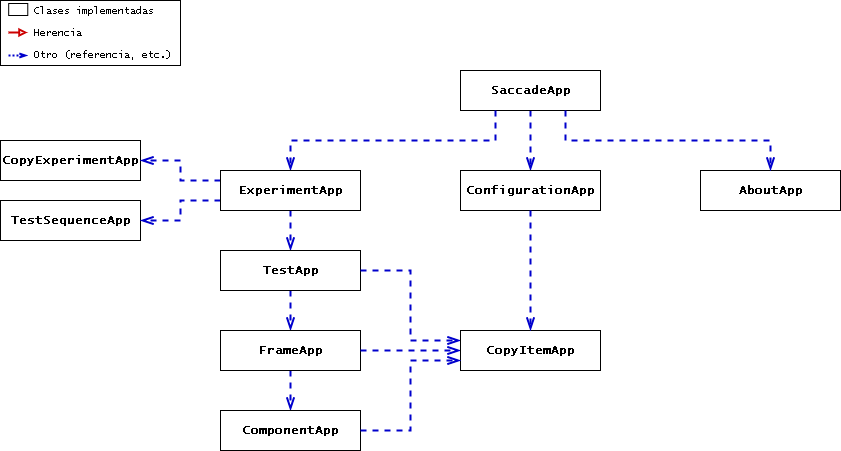
\includegraphics[width=\textwidth]{cap_03_gui_class_tree}
				\caption{Diagrama de clases de la \textit{GUI}.}
				\label{fig:03_gui_class_tree}
			\end{figure} 

			En la figura \ref{fig:03_gui_class_tree} se aprecia un diagrama simplificado de las clases utilizadas para la construcción de las ventanas que conforman la \textit{GUI}. En las siguientes páginas se presentará, para cada una, una descripción breve de su funcionalidad y se detallarán sus componentes.

			\newpage 
			\begin{enumerate}\setlength\itemsep{-0.5em}
				\item \textbf{\textref{SaccadeApp}:} Ventana principal de la aplicación. Permite revisar los experimentos y perfiles de configuración almacenados en la base de datos, acceder a la documentación y ejecutar experimentos.
				\begin{figure}[H]
					\centering
					\subfloat[Pestaña de experimentos.]{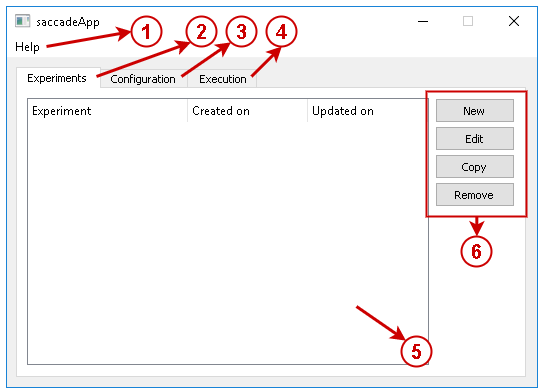
\includegraphics[width=0.51\textwidth]{cap_03_gui_01}}
					\subfloat[Pestaña de configuración.]{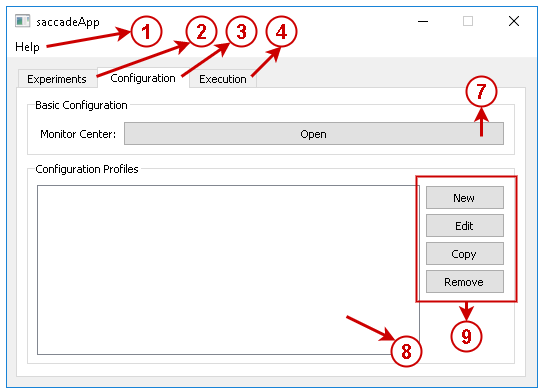
\includegraphics[width=0.51\textwidth]{cap_03_gui_02}}\\
					\subfloat[Pestaña de ejecución.]{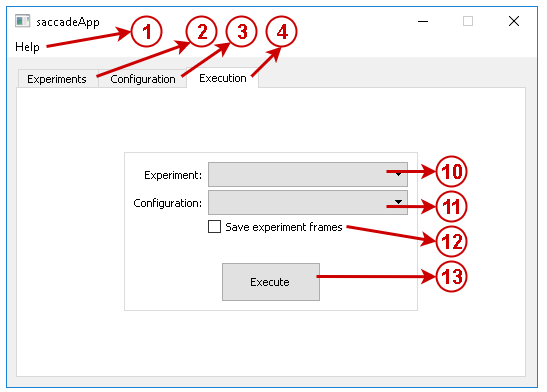
\includegraphics[width=0.51\textwidth]{cap_03_gui_03}}
					\caption{Ventana principal.}
					\label{fig:03_gui_main}
				\end{figure} 

				\vspace{-5mm}

				En la figura \ref{fig:03_gui_main}:
				\begin{enumerate}[(1)]\setlength\itemsep{-0.5em}
					\item Menú de ayuda. Contiene accesos a la documentación de la aplicación (este trabajo de título) y a información de contacto del autor.
					\item Pestaña que contiene los experimentos disponibles. 
					\item Pestaña que contiene los perfiles de configuración. 
					\item Pestaña donde se encuentra el dialogo de ejecución de experimentos. 
					\item Vista de tipo árbol que muestra los experimentos almacenados en la base de datos ordenados por nombre y versión. Se indican también la fecha de creación y la fecha de la última modificación del mismo.  
					\item Permite la manipulación de los experimentos almacenados. 
					\item Acceso al centro de monitores de \textit{psychoPy}.
					\item Lista de los perfiles de configuración almacenados en la base de datos ordenados por nombre.
					\item Permite la manipulación de los perfiles de configuración almacenados.
					\item Lista de experimentos disponibles para ejecución. 
					\item Lista con los perfiles de configuración disponibles. 
					\item Permite escoger si se desea almacenar durante la ejecución capturas de pantalla de los cuadros desplegados en cada experimento.
					\item Permite comenzar la ejecución de un experimento. 
				\end{enumerate}

				\item \textbf{\textref{ExperimentApp}:} Permite revisar y/o configurar un experimento, las tareas que lo componen y la secuencia de ejecución de las mismas. Se puede acceder a ella desde la ventana principal mediante los botones \textref{New} y \textref{Edit} ubicados en la pestaña \textref{Experiments}.
				\begin{figure}[H]
					\centering
					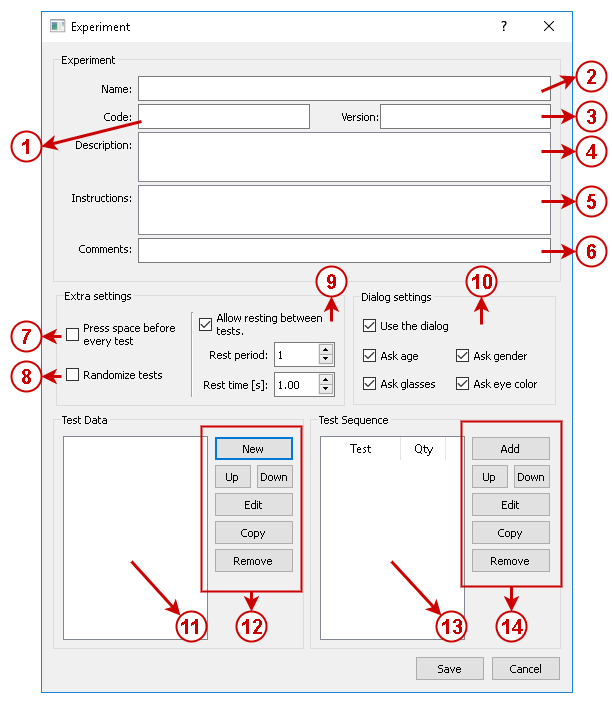
\includegraphics[width=0.5\textwidth]{cap_03_gui_04}
					\caption{Ventana para configuración de experimentos.}
					\label{fig:03_gui_exp}
				\end{figure}

				\vspace{-5mm}

				En la figura \ref{fig:03_gui_exp}:
				\begin{enumerate}[(1)]\setlength\itemsep{-0.5em}
					\item Campo obligatorio, usualmente críptico, que identifica de forma única al experimento. Debe tener entre 3 y 10 caracteres.
					\item Campo obligatorio que identifica de forma breve, más no críptica, un experimento (similar al nombre que se le daría en el título de un \textit{paper}). Debe tener entre 3 y 50 caracteres.
					\item Campo obligatorio que identifica distintas implementaciones o versiones de un tipo de experimento. Debe tener entre 3 y 10 caracteres.
					\item Campo optativo que permite describir de forma más clara la naturaleza y objetivos del experimento.
					\item Campo optativo, a ser presentado al paciente al comienzo de la sesión de experimentación, que describe de forma general el como proceder en las tareas a realizar.
					\item Campo optativo que permite incluir un recordatorio breve para quien realiza la sesión de experimentación. El mensaje puede contener hasta 50 caracteres. 
					\item Permite definir si el paciente debe presionar la tecla espacio antes de la realización de cada tarea. 
					\item Permite presentar las tareas de la secuencia de ejecución de forma aleatoria.
					\item Permite configurar tanto la frecuencia como duración de descansos durante la sesión de experimentación.
					\item Permite incluir algunas preguntas tipo para adquirir más información del paciente. 
					\item Lista con las tareas configuradas para el experimento. 
					\item Permite la manipulación de las tareas configuradas.
					\item Tabla que muestra la secuencia de ejecución del experimento indicando el nombre de la tarea a presentar y el número de repeticiones. 
					\item Permite la manipulación de los elementos de la secuencia. 
				\end{enumerate}

				\item \textbf{\textref{CopyExperimentApp}:} Permite realizar una copia de un experimento existente, para lo cual se requiere obtener un nuevo código y versión. Se puede acceder a ella desde la ventana principal mediante el botón \textref{copy} ubicado en la pestaña \textref{Experiments}.
				\begin{figure}[H]
					\centering
					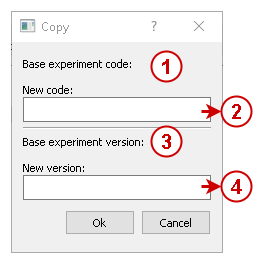
\includegraphics[width=0.32\textwidth]{cap_03_gui_11}
					\caption{Ventana de copia para experimentos.}
					\label{fig:03_gui_exp_cpy}
				\end{figure}

				\vspace{-5mm}

				En la figura \ref{fig:03_gui_exp_cpy}:
				\begin{enumerate}[(1)]\setlength\itemsep{-0.5em}
					\item Muestra el código utilizado en el experimento original.
					\item Campo obligatorio, usualmente críptico, que identifica de forma única al experimento. Debe tener entre 3 y 10 caracteres.
					\item Muestra la versión utilizada en el experimento original.  
					\item Campo obligatorio que identifica distintas implementaciones o versiones de un tipo de experimento. Debe tener entre 3 y 10 caracteres.
				\end{enumerate}

				\item \textbf{\textref{TestSequenceApp}:} Permite la creación de un nuevo elemento para la secuencia de ejecución del experimento. Se puede acceder a ella desde \textref{ExperimentApp} mediante el botón \textref{Add} o \textref{Edit} de la botonera de secuencia. 
				\begin{figure}[H]
					\centering
					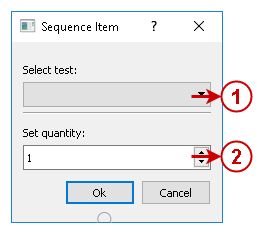
\includegraphics[width=0.32\textwidth]{cap_03_gui_09}
					\caption{Ventana de configuración para secuencia de ejecución del experimento.}
					\label{fig:03_gui_exp_seq}
				\end{figure}

				\vspace{-5mm}

				En la figura \ref{fig:03_gui_exp_seq}:
				\begin{enumerate}[(1)]\setlength\itemsep{-0.5em}
					\item Lista con las tareas disponibles para el experimento.
					\item Campo para ingresar el número de veces que la tarea debe ser ejecutada.
				\end{enumerate}

				\item \textbf{\textref{TestApp}:} Permite revisar y/o configurar una tarea específica y los cuadros que la componen. Se puede acceder a ella desde \textref{ExperimentApp} utilizando los botones \textref{New} y \textref{Edit} de la lista de tareas.
				\begin{figure}[H]
					\centering
					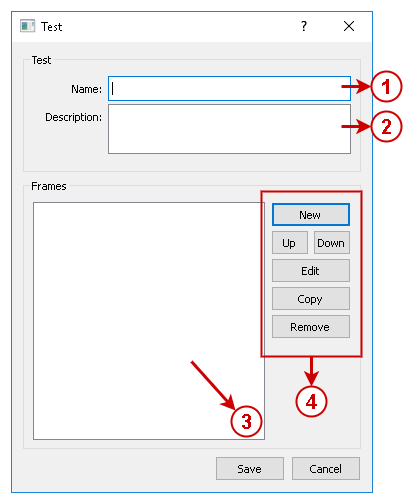
\includegraphics[width=0.5\textwidth]{cap_03_gui_05}
					\caption{Ventana para configuración de tareas.}
					\label{fig:03_gui_tes}
				\end{figure}

				\vspace{-5mm}

				En la figura \ref{fig:03_gui_tes}:
				\begin{enumerate}[(1)]\setlength\itemsep{-0.5em}
					\item Campo obligatorio, identifica de forma única a la tarea dentro de un experimento. Debe tener entre 3 y 50 caracteres.
					\item Campo optativo que permite describir de forma mas clara las características de la tarea.
					\item Lista con los cuadros que componen la tarea.
					\item Permite manipular los cuadros configurados.
				\end{enumerate}

				\item \textbf{\textref{FrameApp}:} Permite revisar y/o configurar un cuadro específico, además de los componentes que lo conforman. Se puede acceder a esta ventana desde \textref{TestApp} utilizando los botones \textref{New} y \textref{Edit} de la lista de cuadros. 
				\begin{figure}[H]
					\centering
					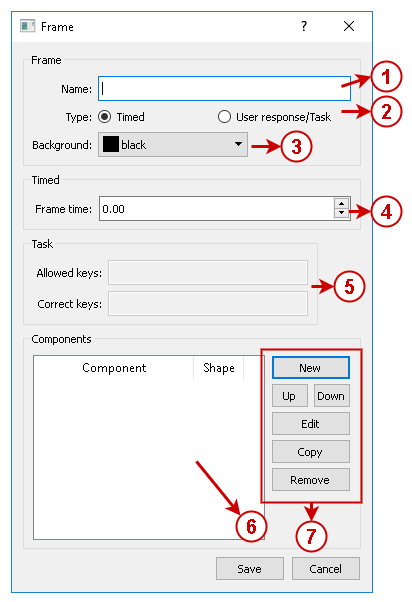
\includegraphics[width=0.5\textwidth]{cap_03_gui_06}
					\caption{Ventana para configuración de cuadros.}
					\label{fig:03_gui_fra}
				\end{figure}

				\vspace{-5mm}

				En la figura \ref{fig:03_gui_fra}:
				\begin{enumerate}[(1)]\setlength\itemsep{-0.5em}
					\item Campo obligatorio, identifica de forma única al cuadro dentro de una tarea. Debe tener entre 3 y 50 caracteres.
					\item Selecciona el tiempo de comportamiento que tendrá el cuadro durante la ejecución.
					\item Permite escoger el color de fondo del cuadro.
					\item Si se selecciona un comportamiento temporizado este campo permite definir por cuanto tiempo, en segundos, se mantendrá el cuadro en pantalla.
					\item En caso de escoger un comportamiento que requiere respuesta de usuario (mediante teclado) estos campos permiten definir tanto las teclas permitidas como, en caso de existir, las que se asocian a respuestas correctas.
					\item Lista que indica tanto los nombres como tipos de forma de los componentes que conforman el cuadro.
					\item Permite manipular los componentes configurados.
				\end{enumerate}

				\item \textbf{\textref{ComponentApp}:} Permite revisar/configurar las características de un componente visual específico. Se puede acceder a esta ventana desde \textref{FrameApp} utilizando los botones \textref{New} o \textref{Edit} de la lista de componentes.
				\begin{figure}[H]
					\centering
					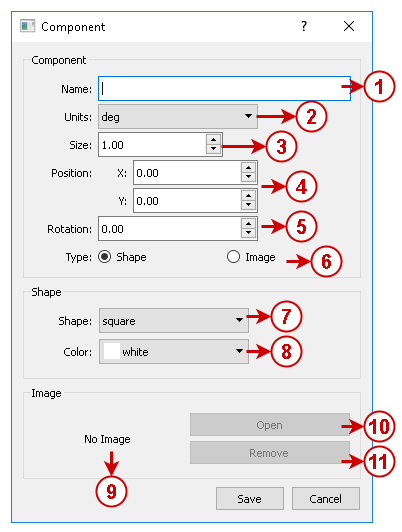
\includegraphics[width=0.5\textwidth]{cap_03_gui_07}
					\caption{Ventana de configuración de componente.}
					\label{fig:03_gui_com}
				\end{figure}

				\vspace{-5mm}

				En la figura \ref{fig:03_gui_com}:
				\begin{enumerate}[(1)]\setlength\itemsep{-0.5em}
					\item Campo obligatorio, identifica de forma única al componente dentro de un cuadro. Debe tener entre 3 y 50 caracteres.
					\item Permite definir el tipo de unidades a utilizar para dibujar el componente.
					\item Tamaño de la figura.
					\item Posición de la figura en el cuadro en base a las unidades de medida seleccionadas.
					\item Permite rotar al componente respecto de su centro.
					\item Selecciona si se trabajará con una figura predeterminada o una imagen.
					\item Permite escoger la figura a utilizar.
					\item Color del relleno y bordes de la figura.
					\item En caso de existir una imagen cargada en el componente esta se muestra en este espacio. Para hacer \textit{zoom} solo es necesario pasar el cursor por encima.
					\item Permite buscar una imagen en el equipo y cargarla en el componente.
					\item Permite eliminar la imagen.
				\end{enumerate}

				\item \textbf{\textref{ConfigurationApp}:} Permite revisar/configurar las características de un perfil de configuración. Se puede acceder a ella desde la ventana principal mediante los botones \textref{New} y \textref{Edit} ubicados en la pestaña \textref{Configuration}.
				\begin{figure}[H]
					\centering
					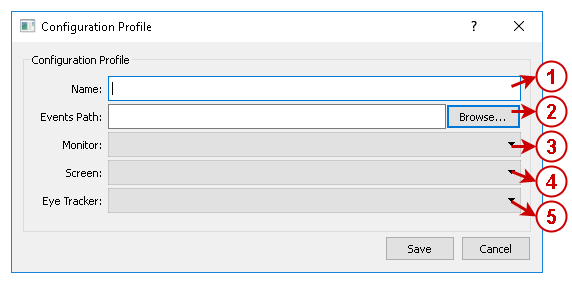
\includegraphics[width=0.6\textwidth]{cap_03_gui_10}
					\caption{Ventana para copia de elementos.}
					\label{fig:03_gui_con}
				\end{figure}

				\vspace{-5mm}

				En la figura \ref{fig:03_gui_con}:
				\begin{enumerate}[(1)]\setlength\itemsep{-0.5em}
					\item Campo obligatorio, identifica de forma única al perfil de configuración. Debe tener entre 3 y 50 caracteres.
					\item Permite definir un directorio para almacenar los resultados obtenidos de la ejecución del experimento.
					\item Lista que muestra los perfiles de configuración de monitor disponibles\footnote{En el \textit{Monitor Center} de \textit{psychoPy}. Es posible acceder a esta herramienta desde \textref{SaccadeApp}, pestaña \textref{Configuration}.}.
					\item Lista que indica las pantallas conectadas y sus dimensiones.
					\item Lista que indica las configuraciones disponibles de \textit{eye tracker}.
				\end{enumerate}

				\item \textbf{\textref{CopyItemApp}:} Esta ventana se usa en los procesos de copia de tareas, cuadros, componentes y perfiles de configuración para determinar el nombre del nuevo objeto, que debe cumplir con no estar en la lista contenedora. Esta ventana puede ser accedida al utilizar el botón \textref{Copy} desde \textref{FrameApp}, \textref{TestApp}, \textref{ExperimentApp} y la pestaña \textref{Configuration} en \textref{SaccadeApp}. 
				\begin{figure}[H]
					\centering
					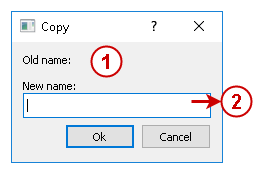
\includegraphics[width=0.32\textwidth]{cap_03_gui_08}
					\caption{Ventana utilizada en el proceso de copia.}
					\label{fig:03_gui_copy}
				\end{figure}

				\vspace{-5mm}

				En la figura \ref{fig:03_gui_copy}:
				\begin{enumerate}[(1)]\setlength\itemsep{-0.5em}
					\item Muestra el nombre del objeto original.
					\item Campo obligatorio que identifica de forma única al objeto a copiar. Debe tener entre 3 y 50 caracteres.
				\end{enumerate}

				\item \textbf{\textref{AboutApp}:} Ventana de información. Indica la versión de la aplicación y datos de contacto del autor.
				\begin{figure}[H]
					\centering
					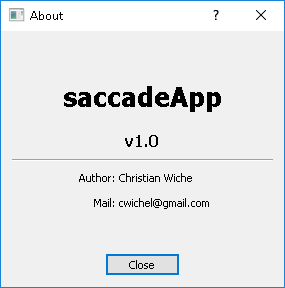
\includegraphics[width=0.32\textwidth]{cap_03_gui_12}
					\caption{Ventana de información.}
					\label{fig:03_gui_about}
				\end{figure}

			\end{enumerate}		 

	% ===============================================================
	% ===============================================================
\end{document}